\documentclass[12pt]{article}
\usepackage[margin=1in]{geometry}
\geometry{letterpaper}                  
\usepackage{float}
\usepackage{graphicx}
\usepackage[hyphens]{url}
\usepackage{fancyhdr}
%\pagestyle{fancy}
\usepackage{fixltx2e}
\usepackage{amsmath,amsfonts,amsthm,amssymb}
\usepackage{graphicx}
\usepackage{algorithm}
\usepackage{algorithmic}
\usepackage{url}
\usepackage[normalem]{ulem}
\usepackage[pdftex]{color}
\usepackage{varioref}
\usepackage{mathrsfs}
\usepackage{amsmath}
\labelformat{equation}{\textup{(#1)}}
\usepackage[sort&compress,colon,square,numbers]{natbib}


\begin{document}

\begin{center}\Large \bf EN.580.694: Statistical Connectomics \\ Final Project Report \end{center}
\begin{center} akim1 $\cdot$  \today \end{center}
\bigskip

\section*{Effects of Spatial Resolution on Accurate Determination of Graph Connectivitiy}
$\\ \\$
\begin{figure}[H]
\centering
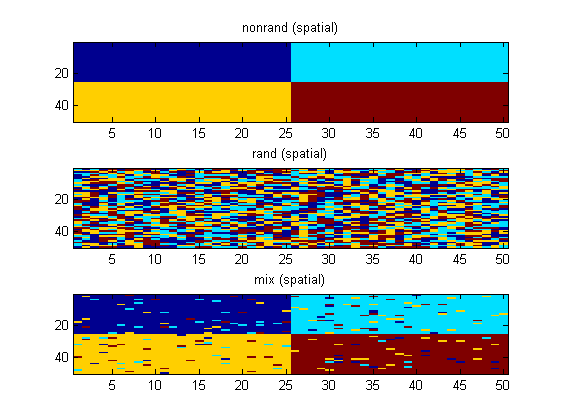
\includegraphics{Fig1.png}
\caption{2-dimensional grid with block identity of the pixels for the three
different cases: non-random, random, and mixture of two.}
\end{figure}

\begin{figure}[H]
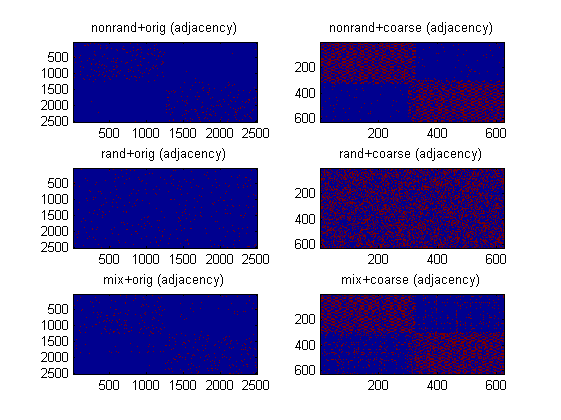
\includegraphics{Fig2.png}
\caption{Representation of the adjacency matrix for non-coarsened and coarsened
data for the three different cases.}
\end{figure}

\begin{figure}[H]
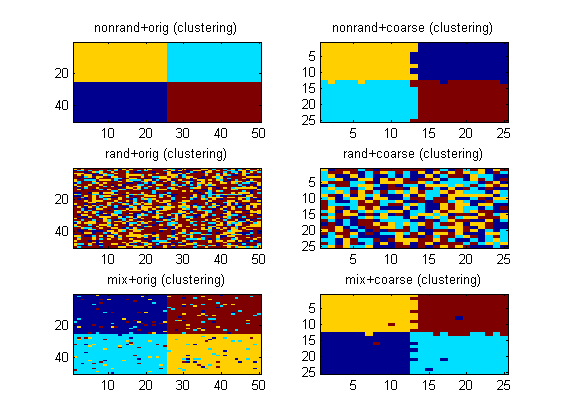
\includegraphics{Fig3.png}
\caption{Result of k-means clustering for non-coarsened and coarsened data for
the three different cases.}
\end{figure}
\newpage

\paragraph{Opportunity}
The ability to measure individual connectomes holds great promise in advancing
our knowledge of the brain and consciousness. Despite these promises, current
technology and state of knowledge prevents the rescaling of this measurement
process into a computational problem that can be solved within a reasonable
time with finite resources. The complexity of the problem inevitably poses a
challenge both in validation of data and establishment of a consensus dataset.
This proposal posits that one factor that may contribute to these challenges is
the spatial resolution at which the data is obtained.

\paragraph{Challenge}
Previous studies have explored the role of resolution in diffusion spectrum MRI
\cite{cammoun2012mapping}. Despite the fact that a voxel is the elementary unit
of MRI imaging, voxels represent information from collections of neurons.
Thus, there exists an inherent loss of information that results from the
observation of aggregate behaviors.  Changes in ``hubs'' of a connectome have
previously been reported to be a characteristic of many diseases of the brain
\cite{crossley2014hubs}. Information of these ``hubs'' can be lost without
sufficient level of resolution, and their activities can be drowned out by the
presence of their neighboring neurons. In this study, a purely computational
approach was taken to study the implications of observing aggregate behavior
and resulting potential information loss.

\paragraph{Action}
A neuron connectivity network was generated based on a stochastic block model.
The block identity of each neuron was assigned based on their relative location
in a 2-dimensional grid. In one limiting case, contiguous pixels were assigned
to one block (nonrand case), while in another limiting case, all pixels were
randomly assigned to a block (rand case). An intermediate case was also
explored where a probability distribution was used to create a mixture of the
two limiting cases (mix case).  Once the connectivity network was generated,
the network was coarsened by combining the spatial and connective properties of
pixels in a two-by-two square into one new pixel. K-means clustering was
performed on this new coarsened grid to qualitatively characterize any notable
losses of information in respect to true information and non-coarsened data.

\paragraph{Resolution}
Representation of the adjacency matrices showed the geometric delineation of
the pixels and their respective connections. Coarsening the 2-dimensional grid
led to a decrease in sparsity as shown across all three different cases.
Subsequently, k-means clustering was used to correctly recapitulate the true
information in the non-random and mixture cases. Whether the true information
was correctly determined in both random cases was difficult to ascertain from
the generated figure. Coarsening the data led to the introduction of artifacts
at the boundaries in the nonrandom and mixture case. This was accompanied by a
significant decrease in the heterogeneity of the region, suggesting that
potentially important neuronal activity is lost in aggregate information.

\paragraph{Future Work}
Much of the work presented in this report was limited by the availability of
the necessary computational resources. Future work would include the expansion
of the analysis into 3-dimensions with significantly greater number of pixels
and inclusion of physiological regions. A rigorous framework would also be
established to determine statistical confidence, and empirical data would be
used to validate these findings.

\newpage

\bibliography{akim1_report.bib}
\bibliographystyle{plain}
\end{document}
